\begin{tabular}{M{7cm}M{10.5cm}}
	\textbf{ĐỀ ÔN TẬP}& \textbf{KỲ THI TỐT NGHIỆP THPT QUỐC GIA}\\
	\textbf{MÃ ĐỀ: 001}& \textbf{Bài thi môn: VẬT LÝ}\\
	\textit{(Đề thi có 04 trang)}& \textit{Thời gian làm bài: 50 phút, không kể thời gian phát đề}
	
	\noindent\rule{4cm}{0.8pt} \\
\end{tabular}
\setcounter{section}{0}
\section{Câu trắc nghiệm nhiều phương án lựa chọn}
\textit{Thí sinh trả lời từ câu 1 đến câu 18. Mỗi câu hỏi thí sinh chọn một phương án}
\setcounter{ex}{0}
\Opensolutionfile{ans}[ans/THPTQG-001-TN]

\Closesolutionfile{ans}
\section{Câu trắc nghiệm đúng/sai} 
\textit{Thí sinh trả lời từ câu 1 đến câu 4. Trong mỗi ý \textbf{a)}, \textbf{b)}, \textbf{c)}, \textbf{d)} ở mỗi câu, thí sinh chọn đúng hoặc sai}
\setcounter{ex}{0}
\Opensolutionfile{ans}[ans/THPTQG-001-TF]
% ===================================================================
\begin{ex}
	Hình 1a biểu diễn sơ đồ của hệ thống làm mát động cơ ô tô. Trong một lần thử nghiệm hệ thống này, các số liệu được thống kê vào Bảng 1b. Coi rằng, khi nhiên liệu bị đốt cháy hoàn toàn thì $\SI{30}{\percent}$ nhiệt năng từ nhiên liệu được chuyển thành cơ năng có ích.
	\begin{center}
		\begin{tabular}{M{7cm}M{10cm}}
			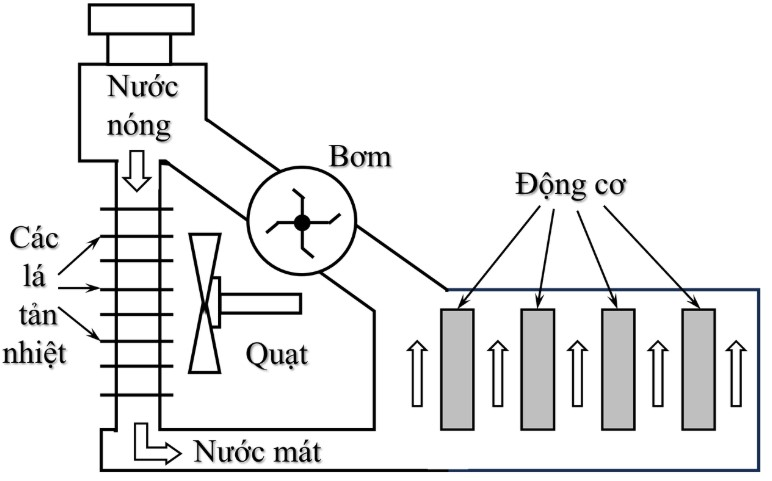
\includegraphics[scale=0.5]{../figs/THPTQG-001-1} &\vspace{-0.75cm} \begin{tabular}{|L{8.2cm}|M{1.3cm}|}
				\hline
				Thời gian thử nghiệm (phút) & $\SI{5.0}{}$\\
				\hline
				Khối lượng nhiên liệu tiêu thụ $\left(\si{\kilogram}\right)$ & $\SI{0.80}{}$\\
				\hline
				Năng suất tỏa nhiệt của nhiên liệu $\left(\si{\joule/\kilogram}\right)$ & $\SI{4.6E7}{}$\\
				\hline
				Lưu lượng dòng nước làm mát $\left(\si{\kilogram/\second}\right)$ & $\SI{0.22}{}$\\
				\hline
				Nhiệt độ của nước mát $\left(\si{\celsius}\right)$ & $\SI{30.0}{}$\\
				\hline
				Nhiệt độ của nước nóng $\left(\si{\celsius}\right)$ & $\SI{80.0}{}$\\
				\hline
				Lưu lượng không khí qua các lá tản nhiệt $\left(\si{\kilogram/\second}\right)$ & $\SI{1.25}{}$\\
				\hline
				Nhiệt độ ban đầu của không khí $\left(\si{\celsius}\right)$ & $\SI{20.0}{}$\\
				\hline
				Nhiệt dung riêng của dầu $\left(\si{\joule/\kilogram\cdot\kelvin}\right)$ & $1800$\\
				\hline
				Nhiệt dung riêng của nước $\left(\si{\joule/\kilogram\cdot\kelvin}\right)$ & $4200$\\
				\hline
					Nhiệt dung riêng của không khí $\left(\si{\joule/\kilogram\cdot\kelvin}\right)$ & $760$\\
				\hline
			\end{tabular}\\
			Hình 1a & Bảng 1b
		\end{tabular}
	\end{center}
	
	\choiceTF
	{Có thể thay nước bằng dầu để tăng hiệu quả làm mát động cơ}
	{Nhiệt lượng hao phí trong quá trình thử nghiệm là $\SI{11.04}{\mega\joule}$}
	{\True Nhiệt lượng nước nóng tỏa ra môi trường qua các lá tản nhiệt là $\SI{13.86}{\meter\joule}$}
	{\True Nếu hiệu suất trao đổi nhiệt lượng giữa nước nóng và không khí $\SI{100}{\percent}$ thì nhiệt độ của dòng không khí đi ra khỏi các lá tản nhiệt là $\SI{68.6}{\celsius}$}
	\loigiai{}
\end{ex}
% ===================================================================
\begin{ex}
	\immini{Một nguồn phóng xạ đặt trong hộp chì phát ra các tia $\alpha$, $\beta^-$, $\gamma$ xuyên qua một lỗ nhỏ trên hộp chì. Một lá nhôm chắn bên ngoài lỗ nhỏ đó, phía sau lá nhôm là vùng không gian có điện trường đều được tạo ra bởi hai tấm kim loại phẳng tích điện trái dấu. Sau khi đi vào điện trường, chùm tia phóng xạ tách thành hai chùm tia a và b. Tia a truyền theo phương ban đầu còn tia b bị lệch như hình vẽ. }
	{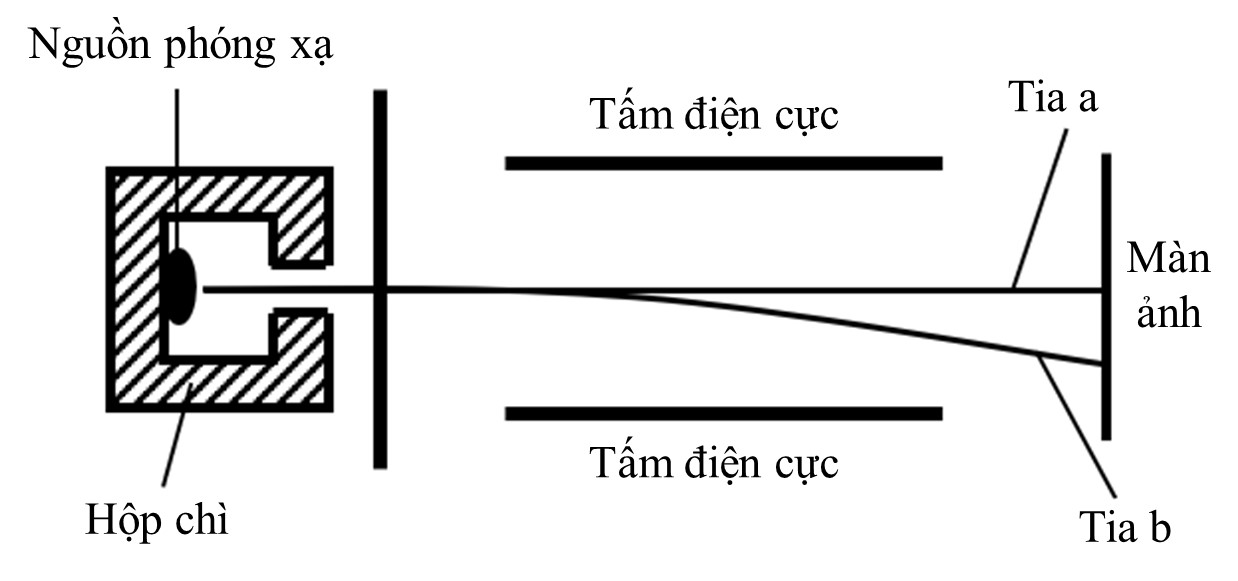
\includegraphics[scale=0.4]{../figs/THPTQG-001-3}}
	\choiceTF
	{Tia a là tia $\alpha$}
	{\True Tia b là tia $\beta^-$}
	{Tấm điện cực phía trên tích điện dương}
	{Có thể thay thế hộp chì bằng hộp sắt để chứa nguồn phóng xạ}
	\loigiai{}
\end{ex}
% ===================================================================
\begin{ex}
	Hình 2a mô phỏng một dynamo gắn trên xe đạp và hình b là cấu tạo của nó. Khi bánh xe quay, núm dẫn động và nam châm cũng quay theo, do đó từ thông qua cuộn dây biến thiên. Lúc này, trong cuộn dây xuất hiện dòng điện cảm ứng và thắp sáng bòng đèn. Dây dẫn được nối với đèn $L_1$ có ghi $\SI{12}{\volt}-\SI{6}{\watt}$. Khi núm dẫn động quay với tốc độ không đổi, điện áp đầu ra của dynamo được coi gần như là dòng điện xoay chiều hình sin. Giả sử điện trở của bóng đèn không đổi và không có hiện tượng trượt giữa núm dẫn động và lốp xe.
	\begin{center}
		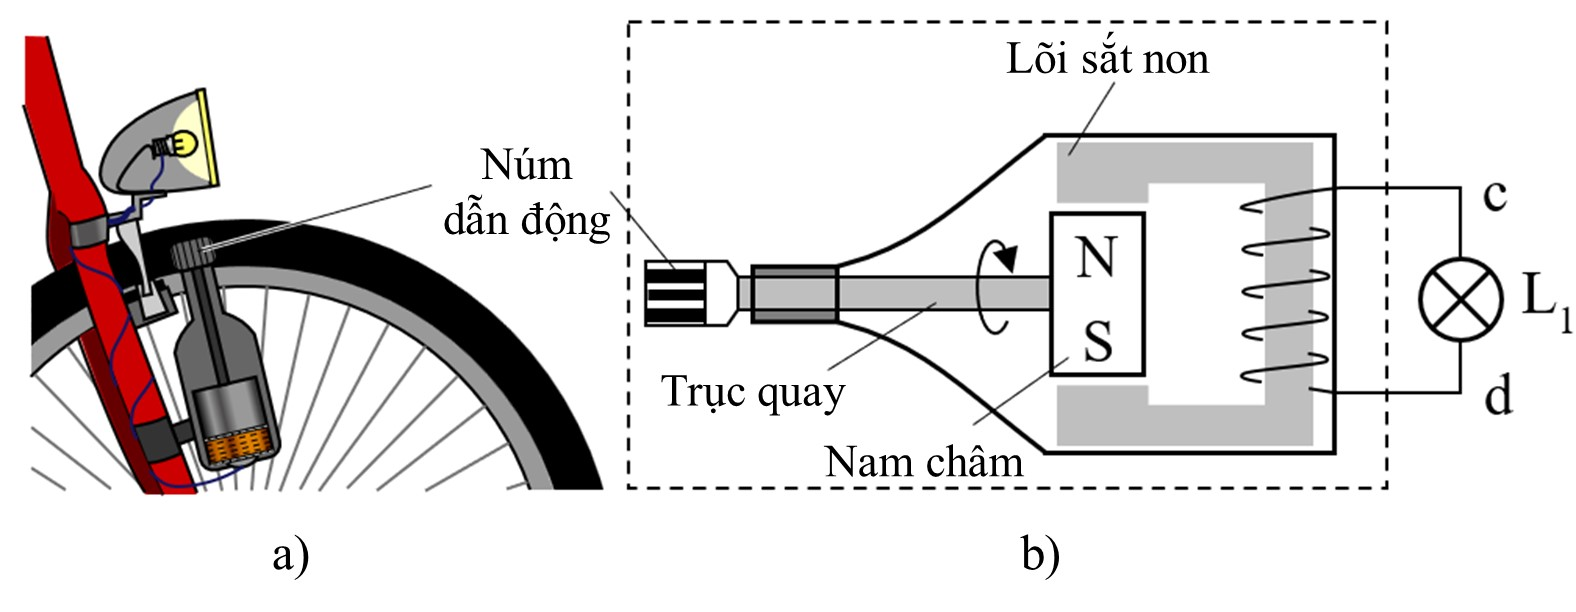
\includegraphics[scale=0.4]{../figs/THPTQG-001-2}\\
		\textit{\textbf{Hình 2.} a) Dynamo trên xe đạp b) Cấu tạo dynamo trên xe đạp.}
	\end{center}
	\choiceTF
	{\True Dynamo hoạt động dựa trên hiện tượng cảm ứng điện từ}
	{\True Khi nam châm quay một góc $\SI{90}{\degree}$ với tốc độ không đổi từ vị trí trên hình thì dòng điện cảm ứng xuất hiện trong cuộn dây có chiều từ d đến c}
	{Trong thời gian nam châm quay một góc $\SI{90}{\degree}$ với tốc độ không đổi từ vị trí trên hình thì dòng điện cảm ứng xuất hiện trong cuộn dây có độ lớn giảm dần}
	{Cho rằng điện trở cuộn dây là $\SI{2}{\ohm}$, khi nam châm quay với tốc độ $\xsi{n}{\text{vòng}/\second}$ thì đèn $L_1$ sáng bình thường. Nếu thay đèn $L_1$ bằng đèn $L_2$ có ghi $\SI{24}{\volt}-\SI{6}{\watt}$ thì điện áp hiệu dụng trên đèn $L_2$ bé hơn $\SI{12}{\volt}$}
	\loigiai{}
\end{ex}

\Closesolutionfile{ans}
\section{Câu trắc nghiệm trả lời ngắn} \textit{Thí sinh trả lời từ câu 1 đến câu 6}\\
\setcounter{ex}{0}
\Opensolutionfile{ans}[ans/THPTQG-001-TL]
% ===============================================================
\begin{ex}
	Nhằm chào mừng ngày lễ Quốc Khánh, Sở Văn hóa và Thể thao TP Hồ Chí Minh đã tổ chức chương trình thả khinh khí cầu vào ngày 02/09/2023. Để một khinh khí cầu có thể bay lên, không khí bên trong nó cần được làm nóng  để làm tăng thể tích, từ đó làm tăng lực nâng của không khí tác dụng lên khí cầu. Trên khinh khí cầu có chở bốn người, tổng khối lượng của khinh khí cầu và người (không tính khối lượng khí bên trong khí cầu) là $\SI{600}{\kilogram}$. Khi không khí bên trong khí cầu được làm nóng và nở ra đến thể tích $\SI{3.0E3}{\meter^3}$ thì khí cầu bắt đầu bay lên. Nhiệt độ không khí bên trong khí cầu khi đó là bao nhiêu $\si{\celsius}$? Giả sử không khí bên ngoài lúc đó có nhiệt độ $\SI{25}{\celsius}$, khối lượng riêng $\SI{1.2}{\kilogram/\meter^3}$, không khí bên trong và bên ngoài khinh khí cầu được coi là khí lý tưởng, khi nung nóng thì không khí bên ngoài khinh khí cầu có nhiệt độ và áp suất không đổi. \textit{(Kết quả làm tròn đến chữ số hàng phần mười)}.
	\shortans[oly]{ }
	\loigiai{
		
	}
\end{ex}
\textit{Sử dụng các thông tin sau cho Câu 2 và Câu 3:}
% ===============================================================
\immini{Thiết bị "cân dòng điện" gồm một khung dây dẫn được đặt trong lòng một ống dây hình trụ như hình vẽ. Dòng điện chạy qua khung dây có cường độ $I_1$. Khi dòng điện chạy qua dây quấn ống dây có cường độ $I_2$ và treo quả nặng khối lượng $m$ ở đầu bên trái của cân thì cân thăng bằng.}
{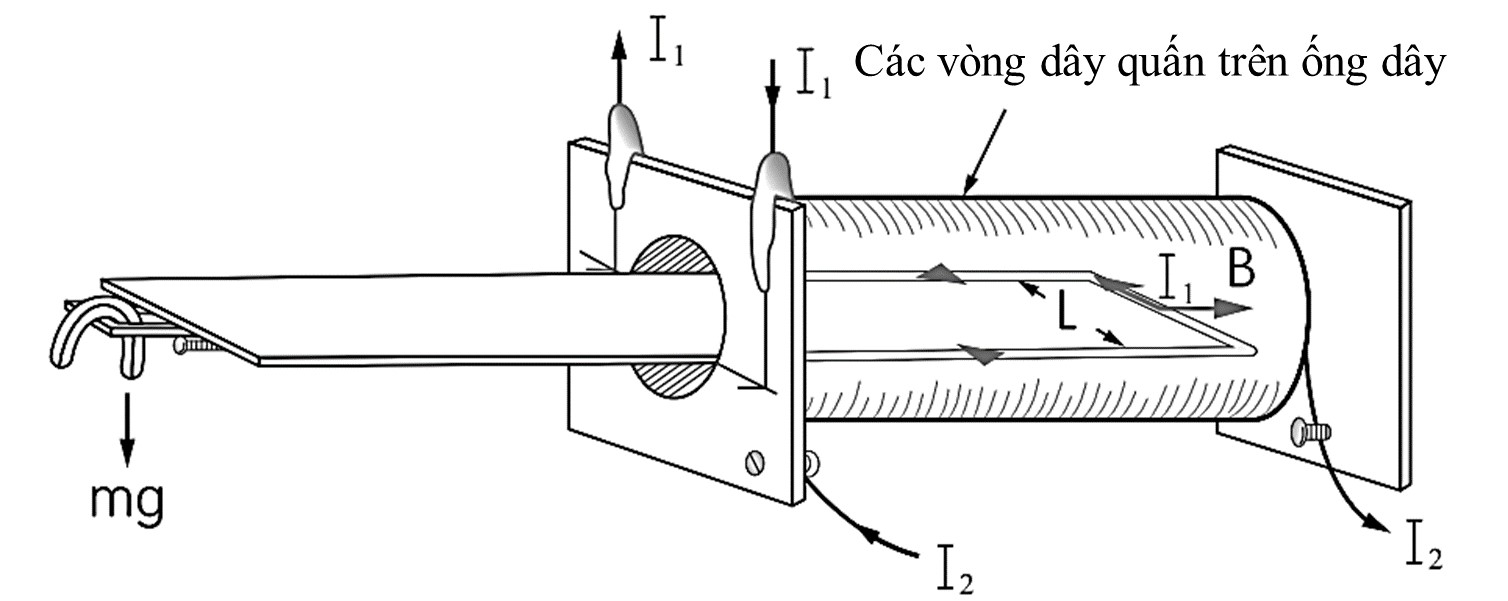
\includegraphics[scale=0.4]{../figs/THPTQG-001-4}}
Biết rằng, độ lớn cảm ứng từ trong lòng ống dây có dòng điện cường độ $I$ chạy qua được xác định bởi $B=\SI{1.26E-6}{}\cdot nI$ với $n$ là số vòng dây quấn trên một đơn vị chiều dài của ống dây.
\begin{ex}
	Nếu dòng điện $I_2$ có cường độ $\SI{1.25}{\ampere}$, đường kính tiết diện dây quấn $d=\SI{0.5}{\milli\meter}$, các vòng dây được quấn sát vào nhau tạo thành 1 lớp dây vừa khít trên chiều dài ống dây thì độ lớn cảm ứng từ trong lòng ống dây là bao nhiêu milli tesla $\left(\si{\milli\tesla}\right)$? \textit{(Kết quả làm tròn đến chữ số hàng phần mười)}.
	\shortans[oly]{$\SI{3.2}{}$}
	\loigiai{
		
	}
\end{ex}
% ===============================================================
\begin{ex}
	Khi thay đổi dòng điện $I_1$ thành $-4I_2$, đồng thời thay đổi dòng điện $I_2$ thành $-I_1/2$ \textit{(dấu "$-$" thể hiện ngược chiều so với dòng điện ban đầu)} thì phải treo ở đầu cân bên trái quả nặng khối lượng $m'$ để cân trở lại trạng thái thăng bằng. Xác định tỉ số $m'/m$.
	\shortans[oly]{2}
	\loigiai{
		
	}
\end{ex}
\textit{Sử dụng các thông tin sau cho Câu 4 đến Câu 6:}\\
Sự cố hạt nhân diễn ra vào ngày 25 tháng 4 năm 1986 tại nhà máy điện hạt nhân Chernobyl ở Pripyat, Cộng hòa Xã hội chủ nghĩa Xô viết Ukraina được coi là thảm họa hạt nhân tồi tệ nhất trong lịch sử. Do không có tường chắn, lượng lớn phóng xạ từ nhà máy lan rộng ra nhiều vùng phía tây Liên bang Xô viết, Đông Âu và Tây Âu, Scandinavia, Anh quốc, và đông Hoa Kỳ. Người ta ước tính rằng thảm họa Chernobyl đã giải phóng khoảng $\SI{6.0}{\mega ci} \ce{^{137}Cs}$ vào môi trường. Biết rằng $\ce{^{137}Cs}$ có chu kì bán rã 30,2 năm. Cho:	
\begin{itemize}
	\item $\SI{1}{Ci}=\SI{3.7E10}{\becquerel}$;
	\item 1 năm $\approx\SI{3.16E7}{\second}$;
	\item số Avogadro $N_A=\SI{6.022E23}{\mole^{-1}}$.
\end{itemize}
% ===============================================================
\begin{ex}
Hằng số phóng xạ của $\ce{^{137}Cs}$ là $\xsi{x\cdot10^{-10}}{\second^{-1}}$. Tìm giá trị của $x$. \textit{(Kết quả làm tròn đến chữ số hàng phần mười)}.
	\shortans[oly]{$\SI{7.3}{}$}
	\loigiai{
		
	}
\end{ex}
% ===============================================================
\begin{ex}
	Xác định khối lượng $\ce{^{137}Cs}$ bị giải phóng \textit{(kết quả tính theo đơn vị kilogram và làm tròn đến chữ số hàng phần mười)}.
	\shortans[oly]{$\SI{69.5}{}$}
	\loigiai{
		
	}
\end{ex}
% ===============================================================
\begin{ex}
	Nếu độ an toàn phóng xạ là $\SI{10.0}{\text{phân rã}/\minute}$ thì sau bao nhiêu năm kể từ thời điểm xảy ra sự cố, con người có thể sinh sống ở khu vực này? \textit{(Kết quả làm tròn đến chữ số hàng đơn vị)}.
	\shortans[oly]{1818}
	\loigiai{
		
	}
\end{ex}
\Closesolutionfile{ans}
\begin{center}
	\textbf{--- HẾT ---}
\end{center}
